\documentclass{beamer}
\usepackage{multicol,lipsum,caption}
\usepackage{mathtools, amsmath,booktabs,verbatim,multicol} 
\usepackage{tikz, pgf, graphicx}
\usetikzlibrary{shapes.geometric, arrows,positioning,matrix,calc,intersections}
%\usepackage{mathptmx}

\usetheme[progressbar=frametitle]{metropolis}
\setbeamertemplate{frame numbering}[fraction]
\useoutertheme{metropolis}
\useinnertheme{metropolis}
\usefonttheme{metropolis}
\usecolortheme{spruce}
\setbeamercolor{background canvas}{bg=white}

\title{Modeling of angle ply laminates using artificial neural network}
\author{Huiyao Zhang}
\institute{Kyoto Institue of Technology}
\date{12-10-2020}
\setbeamertemplate{itemize/enumerate body begin}{\large}

\DeclarePairedDelimiter\Floor\lfloor\rfloor
\DeclarePairedDelimiter\Ceil\lceil\rceil
\begin{document}
\begin{frame}
    \titlepage
\end{frame}




\begin{frame}{2. Neural Work}
    \begin{columns}[c]
    \begin{column}{1\textwidth}
		\begin{figure}
		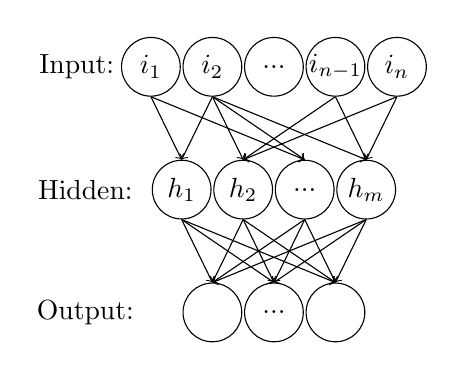
\begin{tikzpicture}
		[ plain/.style={ draw=none, fill=none, }, remember picture, net/.style={ matrix of nodes, nodes={ draw, circle,
			inner sep=7.5pt
			},
		  nodes in empty cells,
		  column sep=-10.5pt,
		  row sep=0.8cm
		  }
		]
		%\draw[help lines] (-3cm,-6cm) grid (6cm,3cm);
		\matrix[net, ampersand replacement=\&] (mat)
		{
					  \& |[plain]| \&           \& |[plain]|  \&           \& |[plain]| \&           \&  |[plain]|      \&               \\
			|[plain]| \&           \& |[plain]| \&            \& |[plain]| \&           \& |[plain]| \&                 \& |[plain]|     \\ 
			|[plain]| \& |[plain]| \&           \& |[plain]|  \&           \& |[plain]| \& 	  	   \&  |[plain]|      \& |[plain]|     \\ 
		  };

		  \node at ($(mat-1-1.west)+(-16pt,0)$) {Input: };
		  \node at ($(mat-2-2.west)+(-24pt,0)$) {Hidden:};
		  \node at ($(mat-3-2.west)+(-24pt,0)$) {Output:};
		  \node at (mat-1-1.base) {$i_1$};
		  \node at (mat-1-3.base) {$i_2$};
		  \node at (mat-1-5.base) {...};
		  \node at (mat-1-7.base) {$i_{n-1}$};
		  \node at (mat-1-9.base) {$i_{n}$};
		  \node at (mat-2-2.base) {$h_1$};
		  \node at (mat-2-4.base) {$h_2$};
		  \node at (mat-2-6.base) {$...$};
		  \node at (mat-2-8.base) {$h_{m}$};
		  \node at (mat-3-5.base) {$...$};

		 \foreach \a in {1,3}{
			\foreach \b in {2,6}{
				\draw[->] (mat-1-\a.south) -- (mat-2-\b.north);
			 }
		  }
		 \foreach \a in {3,7,9}{
			\foreach \b in {4,8}{
				\draw[->] (mat-1-\a.south) -- (mat-2-\b.north);
			 }
		  }

		 \foreach \c in {2,4,6,8}{
			\foreach \d in {3,5,7}{
				\draw[->] (mat-2-\c.south) -- (mat-3-\d.north);
			}
		 }
		\end{tikzpicture}
		\caption{Neural Network Model}
		\end{figure}
    \end{column}
\end{columns}
\end{frame}

\begin{frame}{2. Genetic Algorithm}
    \begin{columns}[c]
    \begin{column}{1\textwidth}

		\begin{figure}
		\centering
		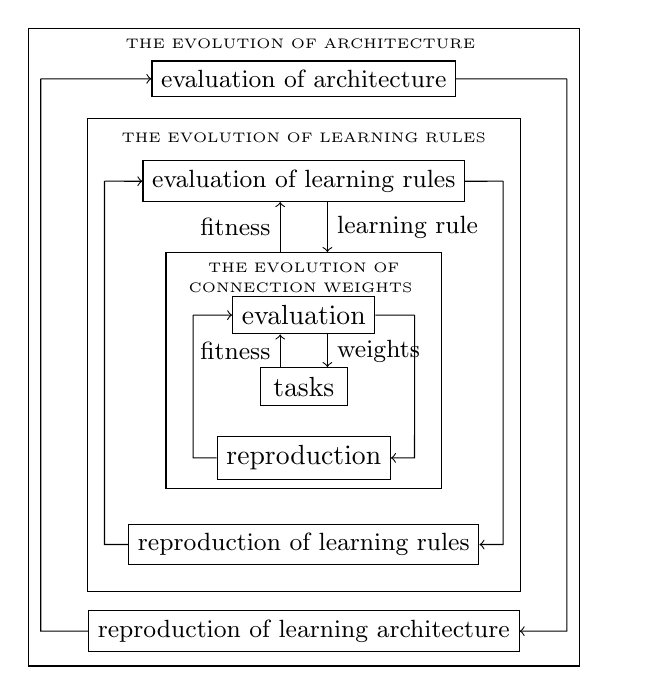
\begin{tikzpicture}
			%\draw[help lines] (-3cm,-6cm) grid (6cm, 6cm);
			\tikzstyle{block} = [rectangle, text centered, draw=black,
			minimum width=1.1cm, minimum height=0.4cm]
			% first level
			\node (evaluation-parent) [block, minimum width=2.4cm, minimum
				height=1.8cm,draw=white] {};
			\node (evaluation) [block] at ($(evaluation-parent.north)$) {evaluation};
			\node (reproduction) [block] at ($(evaluation-parent.south)$) {reproduction};
			\node (tasks) [block, minimum width=1.1cm, minimum height=0.4cm] {tasks};

			\draw[->] ($(evaluation.south)+(0.3cm,0cm)$) --
				($(tasks.north)+(0.3cm,0cm)$) node[auto=left, pos=0.5] {\small weights}; 
			\draw[<-] ($(evaluation.south)+(-0.3cm,0cm)$) --
				($(tasks.north)+(-0.3cm,0cm)$) node[auto=right, pos=0.5] {\small fitness}; 

			% get intersection
			\draw[white] (evaluation.west) coordinate (A) -- ++(-1.5cm,0) coordinate (B);
			\draw[white] (reproduction.west) -- ++(-0.3cm,0) coordinate (C) -- ++(0,4cm) coordinate
				(D);
			\draw[black] (reproduction.west) -- ++(-0.3cm,0) -- (intersection cs:
				first line={(A)--(B)}, second line={(C)--(D)}) coordinate (E);
			\draw[->] (E) -- (evaluation.west);

			\draw[white] (evaluation.east) coordinate (E) -- ++(2cm,0) coordinate (F);
			\draw[white] (reproduction.east) -- ++(0.3cm,0) coordinate (G) -- ++(0,4cm) coordinate
				(H);
			\draw[<-] (reproduction.east) -- ++(0.3cm,0) -- (intersection cs:
				first line={(E)--(F)}, second line={(G)--(H)}) coordinate (I);
			\draw (I) -- (evaluation.east);

			% second level
			\node (level2) [block,draw=black, minimum width=3.5cm, minimum height=3.0cm] at
				(0cm,0.2cm) {};
			\node [align=left] at ($(level2.north)+(0,-0.2cm)$) {\tiny THE EVOLUTION
				OF};
			\node [align=left] at ($(level2.north)+(0,-0.45cm)$) {\tiny CONNECTION
					WEIGHTS 
				};
			% third level
			\node (level3-assister) [block, draw=white, minimum width=5cm, minimum
				height=4.6cm] at
				(0, 0.3cm)  {};
			\node (evaluation) [block] at ($(level3-assister.north)$) {\small evaluation of
				learning rules};
			\node (reproduction) [block] at ($(level3-assister.south)$) {\small reproduction of
				learning rules};

			\draw[->] ($(evaluation.south)+(0.3cm,0cm)$) --
				($(level2.north)+(0.3cm,0cm)$) node[auto=left, pos=0.5] {\small learning
				rule}; 
			\draw[<-] ($(evaluation.south)+(-0.3cm,0cm)$) --
				($(level2.north)+(-0.3cm,0cm)$) node[auto=right, pos=0.5] {\small fitness}; 

			\draw[white] (evaluation.west) coordinate (A) -- ++(-1.3cm,0) coordinate (B);
			\draw[white] (reproduction.west) -- ++(-0.3cm,0) coordinate (C) -- ++(0,4cm) coordinate
				(D);
			\draw[black] (reproduction.west) -- ++(-0.3cm,0) -- (intersection cs:
				first line={(A)--(B)}, second line={(C)--(D)}) coordinate (E);
			\draw[->] (E) -- (evaluation.west);

			\draw[white] (evaluation.east) coordinate (E) -- ++(2cm,0) coordinate (F);
			\draw[white] (reproduction.east) -- ++(0.3cm,0) coordinate (G) -- ++(0,4cm) coordinate
				(H);
			\draw[<-] (reproduction.east) -- ++(0.3cm,0) -- (intersection cs:
				first line={(E)--(F)}, second line={(G)--(H)}) coordinate (I);
			\draw (I) -- (evaluation.east);
		   % fourth level
			\node (level4) [block, draw=black, minimum width=5.5cm, minimum
				height=6.0cm] at
				(0, 0.4cm)  {};
			\node [align=left] at ($(level4.north)+(0,-0.25cm)$) {\tiny THE EVOLUTION
				OF LEARNING RULES};
			% level five
			\node (level5-assister) [block, draw=white, minimum width=6.4cm, minimum
				height=7.0cm] at
				(0, 0.4cm)  {};
			\node (evaluation) [block] at ($(level5-assister.north)$) {\small evaluation of
				architecture};
			\node (reproduction) [block] at ($(level5-assister.south)$) {\small reproduction of
				learning architecture};

			\draw[white] (evaluation.west) coordinate (A) -- ++(-1.5cm,0) coordinate (B);
			\draw[white] (reproduction.west) -- ++(-0.6cm,0) coordinate (C) -- ++(0,4cm) coordinate
				(D);
			\draw[black] (reproduction.west) -- ++(-0.6cm,0) -- (intersection cs:
				first line={(A)--(B)}, second line={(C)--(D)}) coordinate (E);
			\draw[->] (E) -- (evaluation.west);

			\draw[white] (evaluation.east) coordinate (E) -- ++(2cm,0) coordinate (F);
			\draw[white] (reproduction.east) -- ++(0.6cm,0) coordinate (G) -- ++(0,4cm) coordinate
				(H);
			\draw[<-] (reproduction.east) -- ++(0.6cm,0) -- (intersection cs:
				first line={(E)--(F)}, second line={(G)--(H)}) coordinate (I);
			\draw (I) -- (evaluation.east);
			% level 6
			\node (level6) [block, minimum width=7.0cm, minimum
				height=8.1cm] at
				(0, 0.5cm)  {};
			\node [align=left] at ($(level6.north)+(0,-0.2cm)$) {\tiny THE EVOLUTION OF
					ARCHITECTURE
				};
		\end{tikzpicture}
		\caption{Genetic algorithm and artificial neural network}
		\end{figure}
    \end{column}
\end{columns}
\end{frame}


\begin{frame}{2. Classic Lamination Theory}
    \begin{columns}[c]
    \begin{column}{0.5\textwidth}
		\begin{figure}
		\centering
		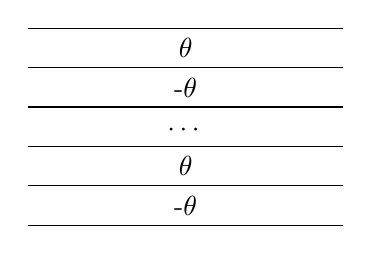
\begin{tikzpicture}
			\draw (0,0) -- (4,0);
			\draw (0,-0.5) -- (4,-0.5) node[midway, above] {$\theta$};
			\draw (0,-1) -- (4,-1) node[midway, above] {\text{-}$\theta$};
			\draw (0,-1.5) -- (4,-1.5) node[midway, above] {$\cdots$};
			\draw (0,-2) -- (4,-2) node[midway, above] {$\theta$};
			\draw (0,-2.5) -- (4,-2.5) node[midway, above] {\text{-}$\theta$};
		\end{tikzpicture}
		\caption{Model for Angle ply laminate}
		\end{figure}
    \end{column}
	\begin{column}{0.5\textwidth}

	\begin{equation} \label{eq:force_and_moments}
		\begin{array}{l}
			\begin{aligned}
		\begin{bmatrix}
			N_x \\
			N_y \\
			N_{xy}
		\end{bmatrix}
		&=
		\begin{bmatrix}
			A_{11} & A_{12} & A_{16} \\
			A_{12} & A_{22} & A_{26} \\
			A_{16} & A_{26} & A_{66} 
		\end{bmatrix}
		\begin{bmatrix}
			\varepsilon_x^0 \\
			\varepsilon_y^0 \\
			\gamma_{xy}^0
		\end{bmatrix}   \\
		&+               
		\begin{bmatrix}
			B_{11} & B_{12} & B_{16} \\
			B_{11} & B_{12} & B_{16} \\
			B_{16} & B_{26} & B_{66} 
		\end{bmatrix}
		\begin{bmatrix}
			k_x \\
			k_y \\
			k_{xy} 
		\end{bmatrix}  \\
	\end{aligned} \\ \\
	\begin{aligned}
		\begin{bmatrix}
			M_x \\
			M_y \\
			M_{xy}
		\end{bmatrix}
		&=
		\begin{bmatrix}
			B_{11} & B_{12} & B_{16} \\
			B_{12} & B_{22} & B_{26} \\
			B_{16} & B_{26} & B_{66} 
		\end{bmatrix}
		\begin{bmatrix}
			\varepsilon_x^0 \\
			\varepsilon_y^0 \\
			\gamma_{xy}^0
		\end{bmatrix} \\ 
		&+  
		\begin{bmatrix}
			D_{11} & D_{12} & D_{16} \\
			D_{11} & D_{12} & D_{16} \\
			D_{16} & D_{26} & D_{66} 
		\end{bmatrix}
		\begin{bmatrix}
			k_x \\
			k_y \\
			k_{xy} 
		\end{bmatrix}
	\end{aligned}
		\end{array}
	\end{equation}
	\end{column}
\end{columns}
\end{frame}


\begin{frame}{2. Methdology}
    \begin{columns}[c]
    \begin{column}{1\textwidth}
	 	\begin{figure}
			\centering
			\resizebox{0.9\linewidth}{!}{
				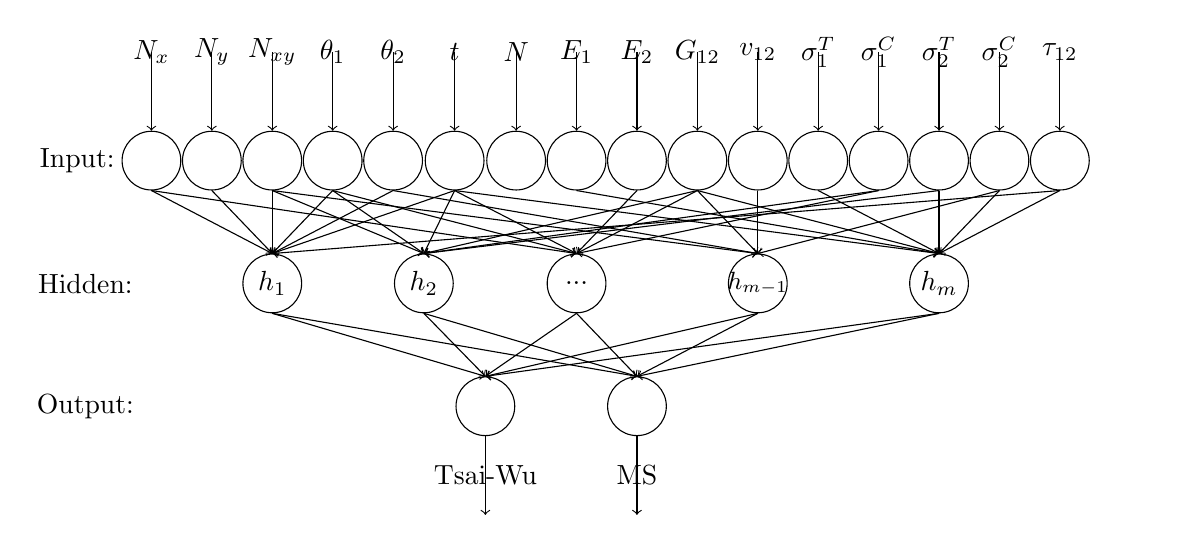
\begin{tikzpicture}
				[ p/.style={ draw=none, fill=none, }, remember picture, 
				  net/.style={ matrix of nodes, nodes={ draw, circle, inner sep=7.5pt },
				  nodes in empty cells,
				  column sep=-10.5pt,
				  row sep=0.8cm
				  }
				]
				%\draw[help lines] (-3cm,-6cm) grid (6cm,3cm);
				\matrix[net,ampersand replacement=\&] (mat)
				{
					  \& |[p]| \&  \& |[p]| \&  \& |[p]| \&  \& |[p]| \&  \& |[p]| \&  \& |[p]| \&  \& |[p]| \&  \& |[p]| \&  \&
						|[p]| \&  \& |[p]| \&  \& |[p]| \&  \& |[p]| \&  \& |[p]| \&  \& |[p]| \&  \& |[p]| \&  \& |[p]|    \\
				 |[p]| \& |[p]| \& |[p]| \&  |[p]| \&        \& |[p]| \& |[p]| \& |[p]| \&|[p]| \&       \& |[p]| \&  |[p]| \& |[p]| \&
				 |[p]| \&       \& |[p]| \&  |[p]| \&  |[p]| \& |[p]| \& |[p]| \&       \&|[p]| \& |[p]| \& |[p]| \& |[p]|
					   \& |[p]| \&       \&  |[p]| \&  |[p]| \& |[p]| \& |[p]| \& |[p]| \&|[p]| \\ 
				 |[p]| \&  |[p]| \& |[p]|  \&  |[p]| \& |[p]|  \&  |[p]| \&  |[p]| \&  |[p]| \& |[p]| \& |[p]| \& |[p]| \&       \& |[p]|
					   \&  |[p]| \& |[p]|  \&  |[p]| \&        \&  |[p]| \&  |[p]| \&  |[p]| \& |[p]| \& |[p]| \& |[p]| \& |[p]| \&     |[p]|
					   \&  |[p]| \& |[p]|  \&  |[p]| \& |[p]|  \&  |[p]| \&  |[p]| \&  |[p]| \\ 
				  };
				  \draw[<-] (mat-1-1.north) --  ++(0,1) node {$N_x$};
				  \draw[<-] (mat-1-3.north) --  ++(0,1) node {$N_y$};
				  \draw[<-] (mat-1-5.north) --  ++(0,1) node {$N_{xy}$};
				  \draw[<-] (mat-1-7.north) --  ++(0,1) node {$\theta_1$};
				  \draw[<-] (mat-1-9.north) --  ++(0,1) node {$\theta_2$};
				  \draw[<-] (mat-1-11.north) --  ++(0,1) node {$t$};
				  \draw[<-] (mat-1-13.north) --  ++(0,1) node {$N$};
				  \draw[<-] (mat-1-15.north) --  ++(0,1) node {$E_1$};
				  \draw[<-] (mat-1-17.north) --  ++(0,1) node {$E_2$};
				  \draw[<-] (mat-1-19.north) --  ++(0,1) node {$G_{12}$};
				  \draw[<-] (mat-1-21.north) --  ++(0,1) node {$v_{12}$};
				  \draw[<-] (mat-1-23.north) --  ++(0,1) node {$\sigma_1^T$};
				  \draw[<-] (mat-1-25.north) --  ++(0,1) node {$\sigma_1^C$};
				  \draw[<-] (mat-1-27.north) --  ++(0,1) node {$\sigma_2^T$};
				  \draw[<-] (mat-1-29.north) --  ++(0,1) node {$\sigma_2^C$};
				  \draw[<-] (mat-1-31.north) --  ++(0,1) node {$\tau_{12}$};
				  \draw[->] (mat-3-12.south) --  ++(0,-1) node[pos=0.5, swap] {Tsai-Wu};
				  \draw[->] (mat-3-17.south) --  ++(0,-1) node[pos=0.5, swap] {MS};
				  \node at ($(mat-1-1.west)+(-16pt,0)$) {Input: };
				  \node at ($(mat-2-2.west)+(-24pt,0)$) {Hidden:};
				  \node at ($(mat-3-2.west)+(-24pt,0)$) {Output:};
				  \node at (mat-2-5.base) {$h_1$};
				  \node at (mat-2-10.base) {$h_2$};
				  \node at (mat-2-15.base) {$...$};
				  \node at (mat-2-21.base) {\small{$h_{m-1}$}};
				  \node at (mat-2-27.base) {$h_{m}$};
				 \foreach \a in {1,3,5,7,9,11,31}{
						\draw[->] (mat-1-\a.south) -- (mat-2-5.north);
					 }
				 \foreach \a in {5,7,11,19,25,27}{
						\draw[->] (mat-1-\a.south) -- (mat-2-10.north);
					 }
				 \foreach \a in {1,7,11,17,19,25}{
						\draw[->] (mat-1-\a.south) -- (mat-2-15.north);
					 }
				 \foreach \a in {5,9,19,21,29}{
						\draw[->] (mat-1-\a.south) -- (mat-2-21.north);
					 }
				 \foreach \a in {11,15,19,23,27,29,31}{
						\draw[->] (mat-1-\a.south) -- (mat-2-27.north);
					 }
				 \foreach \c in {5,10,15,21,27}{
					\foreach \d in {12,17}{
						\draw[->] (mat-2-\c.south) -- (mat-3-\d.north);
					}
				 }
				\end{tikzpicture}
			}
			\caption{Neural Network Model}
		\end{figure}
    \end{column}
\end{columns}
\end{frame}

\begin{frame}{3. Implementation: Data Preparation}
	\begin{table}	
		\begin{tabular}{cccc|cc}
			\toprule
			\multicolumn{4}{c}{\textbf{Input}} &  \multicolumn{2}{c}{\textbf{Output}} \\
			\midrule
			Load  &  Laminate  & Material & Failure  & MS & Tsai-Wu \\
			      &  Structure & Property & Property &    &         \\
			\midrule
			\tiny{120,5,0} &  \tiny{10,-10,8,1.27} &  \tiny{38.6,8.27,0.26,4.14} &  \tiny{1062.0,610.0,31,118,72} &  \tiny{0.068} &\tiny{ 0.062}\\
			\tiny{120,5,0} &  \tiny{10,-10,2,1.27} &  \tiny{38.6,8.27,0.26,4.14} &  \tiny{1062.0,610.0,31,118,72} &  \tiny{1.69}  &\tiny{ 2.18}\\
			\tiny{...}     &   \tiny{...}          & \tiny{...}                  &  \tiny{...}                    &  \tiny{...}  &  \tiny{...}\\
			\tiny{120,5,0} &  \tiny{10,-10,134,1.27} &  \tiny{38.6,8.27,0.26,4.14} &  \tiny{1062.0,610.0,31,118,72} &  \tiny{1.70} &\tiny{1.56 }\\
			\tiny{120,5,0} &  \tiny{10,-10,8,1.27} &  \tiny{181,10.3,0.28,7.17} &  \tiny{1500.0,1500.0,40,246,68} &  \tiny{0.072} &\tiny{ 0.024}\\
			\bottomrule
		\end{tabular}
	\end{table}
\end{frame}

\begin{frame}{4. Implementation: Neural Network}
	\begin{figure}
		\centering
		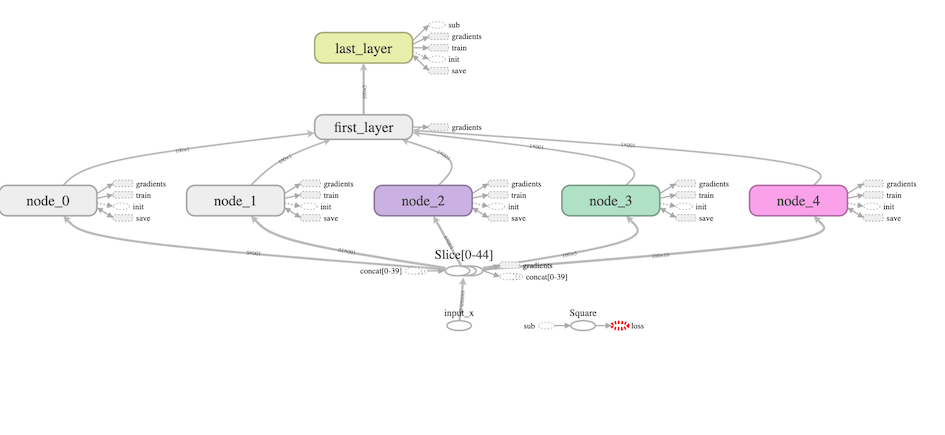
\includegraphics[scale=0.31]{neural-network.png}
	\end{figure}
\end{frame}


\end{document}
